\chapter{Réseaux de neurones et apprentissage profond}

\myminitoc

\paragraph{Motivation}
Les réseaux de neurones viennent d'une volonté d'imiter la biologie. Le cerveau est composé de neurones. Un neurones reçoit des informations des neurones voisins (environs quelques milliers) via des synapses. Les entrées sont approximativement sommées et lorsque cette somme dépasse un certain seuil le neurone envoie un signal électrique via un axone vers le ou les prochains neurones.

\sect{Perceptron}

\paragraph{Neurone formel}
Voici le schéma d'un neurone.
\begin{center}
	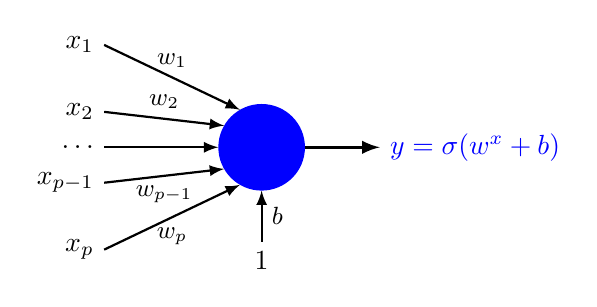
\begin{tikzpicture}[thick, >={latex}]
		\fill[blue] (0, 0) circle(0.55);
		\draw[->] (-2, 1.3) -- node[above] {\small $w_1$} (120:0.55);
		\draw[->] (-2, 0.45) -- node[above] {\small $w_2$} (150:0.55);
		\draw[->] (-2, 0) -- (180:0.55);
		\draw[->] (-2, -0.45) -- node[below] {\small $w_{p-1}$} (210:0.55);
		\draw[->] (-2, -1.3) -- node[below] {\small $w_p$} (240:0.55);
		\node[left] at (-2, 1.3) {$x_1$};
		\node[left] at (-2, 0.45) {$x_2$};
		\node[left] at (-2, 0) {$\dots$};
		\node[left] at (-2, -0.45) {$x_{p-1}$};
		\node[left] at (-2, -1.3) {$x_p$};
		\draw[->, very thick] (0.55, 0) -- (1.5, 0);
		\node[blue, right] at (1.5, 0) {$y = \sigma(w^\trans x + b)$};
		\draw[->] (0, -1.2) -- node[right] {\small $b$} (0, -0.55);
		\node[below] at (0, -1.2) {1};
	\end{tikzpicture}
\end{center}
$x \in \R^p$ est l'entrée du neurone. $w$ est le vecteurs des poids des entrées et $b$ est un biais. $\sigma$ est une fonction d'activation et $y \in \R$ est la sortie du neurone.

\paragraph{Fonction d'activation}
La fonction d'activation doit être non linéaire, non nulle et différentiable. De plus afin d'avoir de bonne performance il est important que la fonction et sa dérivée soient calculables de manière efficace. Voici ci-dessous les fonctions d'activation les plus courantes.

\begin{center}
	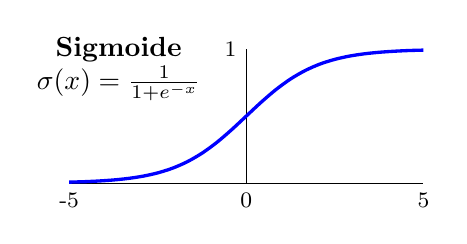
\begin{tikzpicture}[xscale=0.45, yscale=1.7]
		\draw (-5, 0) -- (5, 0);
		\draw (0, 0) -- (0, 1);
		\draw[domain=-5:5, smooth, variable=\x, blue, very thick]
			plot({\x}, {1 / (1 + exp(-\x))});
		\node[below] at (0, 0) {\footnotesize 0};
		\node[below] at (5, 0) {\footnotesize 5};
		\node[below] at (-5, 0) {\footnotesize -5};
		\node[left] at (0, 1) {\footnotesize 1};
		\node at (-3.6, 1) {\textbf{Sigmoide}};
		\node[below] at (-3.6, 0.95) {$\sigma(x) = \frac{1}{1 + e^{-x}}$};
	\end{tikzpicture} \quad
	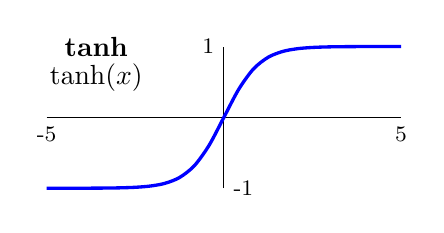
\begin{tikzpicture}[xscale=0.45, yscale=0.9]
		\draw (-5, 0) -- (5, 0);
		\draw (0, -1) -- (0, 1);
		\draw[domain=-5:5, smooth, variable=\x, blue, very thick]
			plot({\x}, {tanh(\x)});
		\node[right] at (0, -1) {\footnotesize -1};
		\node[below] at (5, 0) {\footnotesize 5};
		\node[below] at (-5, 0) {\footnotesize -5};
		\node[left] at (0, 1) {\footnotesize 1};
		\node at (-3.6, 1) {\textbf{tanh}};
		\node[below] at (-3.6, 0.9) {$\tanh(x)$};
	\end{tikzpicture} \quad
	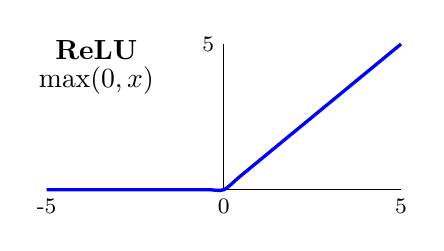
\begin{tikzpicture}[xscale=0.45, yscale=0.37]
		\draw (-5, 0) -- (5, 0);
		\draw (0, 0) -- (0, 5);
		\draw[domain=-5:5, smooth, variable=\x, blue, very thick]
			plot({\x}, {max(0, \x)});
		\node[below] at (0, 0) {\footnotesize 0};
		\node[below] at (5, 0) {\footnotesize 5};
		\node[below] at (-5, 0) {\footnotesize -5};
		\node[left] at (0, 5) {\footnotesize 5};
		\node at (-3.6, 4.8) {\textbf{ReLU}};
		\node[below] at (-3.6, 4.55) {$\max(0, x)$};
	\end{tikzpicture} \\ \vspace{5mm}
	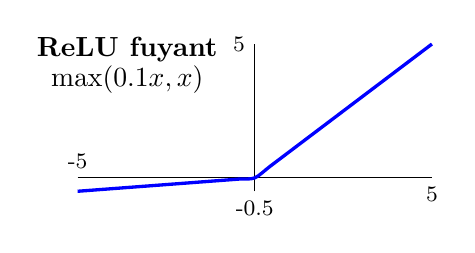
\begin{tikzpicture}[xscale=0.45, yscale=0.34]
		\draw (-5, 0) -- (5, 0);
		\draw (0, -0.5) -- (0, 5);
		\draw[domain=-5:5, smooth, variable=\x, blue, very thick]
			plot({\x}, {max(0.1 * \x, \x)});
		\node[below] at (0, -0.5) {\footnotesize -0.5};
		\node[below] at (5, 0) {\footnotesize 5};
		\node[above] at (-5, 0) {\footnotesize -5};
		\node[left] at (0, 5) {\footnotesize 5};
		\node at (-3.6, 4.8) {\textbf{ReLU fuyant}};
		\node[below] at (-3.6, 4.55) {$\max(0.1 x, x)$};
	\end{tikzpicture} \qquad \qquad
	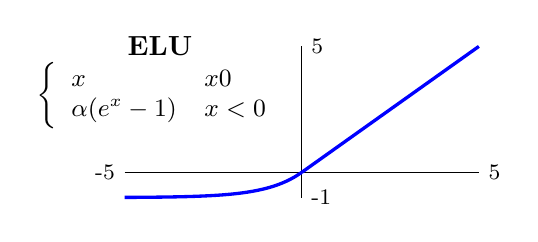
\begin{tikzpicture}[xscale=0.45, yscale=0.32]
		\draw (-5, 0) -- (5, 0);
		\draw (0, -1) -- (0, 5);
		\draw[domain=0:5, smooth, variable=\x, blue, very thick]
			plot({\x}, {\x});
		\draw[domain=-5:0, smooth, variable=\x, blue, very thick]
			plot({\x}, {exp(\x) -1});
		\node[right] at (0, -1) {\footnotesize -1};
		\node[right] at (5, 0) {\footnotesize 5};
		\node[left] at (-5, 0) {\footnotesize -5};
		\node[right] at (0, 5) {\footnotesize 5};
		\node at (-4, 5) {\textbf{ELU}};
		\node[below] at (-4, 4.75) {\small $\left\{ \begin{array}{ll}
			x & x \geqslant 0 \\
			\alpha (e^x - 1) & x < 0
			\end{array} \right.$};
	\end{tikzpicture}
\end{center}

Par la suite on notera l'activation $a = w^\trans x + b$. Puis notera $\Phi$ la fonction de transfert qui étant donné $x$ donne $y$ :
$$ y = \Phi(x) = \sigma(a) = \sigma \left( w^\trans x + b \right) $$
Par la suite on cherche à optimiser $w$ et $b$ pour que dans notre ensemble d'exemples $(x_i, t_i)$, on ai $y_i = \Phi(x_i)$ proche de $t_i$. Pour cela on réalise des descentes de gradient. Comme vu dans un chapitre précédent, on distingue trois descentes différentes :
\begin{itemize}
	\item La descente par batchs qui consiste à sommer les gradients obtenus pour tous les exemples de notre ensemble d'entraîner puis de faire la mise à jour de $w$ et $b$ grâce à cette somme des gradients. Cette méthode est robuste mais lente.
	\item La descente stochastique qui consiste à mettre à jour les poids $w$ et $b$ à chaque exemple. Cette méthode est rapide mais peu robuste.
	\item La descente par mini-batchs qui met à jour les paramètres grâce à une somme de gradients non pas sur tous les exemples mais sur des petits sous-ensembles. Cette descente donne un compromis entre rapidité et robustesse.
\end{itemize}
On rappelle la descente par mini-batchs : \\
\begin{algorithm}
	\caption{Époque de gradient par mini-batch}
	\DontPrintSemicolon
	\KwData{$w, b$ : les paramètres, \\ \qquad \quad
		$\alpha$ : coefficient d'apprentissage, \\ \qquad \quad
		$m$ : taille des mini-batchs}
	$d \gets 0$ \;
	\For{$i = 1, ..., n$}{
		$x_i, t_i \gets $ un exemple $i$ \;
		$d \gets d + \nabla_w loss(w, x_i, t_i)$ \;
		\If{$i \mod m = 0$}{
			$w \gets w - \alpha d$ \;
			$d \gets 0$ \;
		}
	}
\end{algorithm}

\paragraph{Accélération de la descente stochastique}
Il existe plusieurs méthodes qui permettent d'accélérer la descente stochastique :
\begin{itemize}
	\item L'utilisation d'un moment avec un paramètre $\mu < 1$ (ex : $\mu = 0.9$): \vspace{-2mm}
		$$ d \gets \mu d + \nabla_w L(w) \qquad w \gets w - \alpha d $$
	\item L'accélération de Nesterov (ex : $\mu = 0.5$): \vspace{-2mm}
		$$ g_t \gets w - \alpha \nabla_w L(w) \qquad w \gets g_t - \mu (g_t - g_{t-1}) $$
	\item Adaptation du coefficient d'apprentissage : \vspace{-2mm}
		$$ \alpha = \frac{\alpha_0}{\| d \| + \epsilon} \quad \text{où } \epsilon \text{ est très faible, de l'ordre de } 10^{-7} $$
	\item  RMSprop avec $\gamma \in ]0, 1[$ (ex : $\gamma = 0.9$) : \vspace{-2mm}
		$$ g \gets \gamma g + (1 - \gamma) d^\trans d \qquad \alpha = \frac{\alpha_0}{\sqrt{g} + \epsilon} $$
	 \item Adam (ex : $\gamma_1 = 0.9, \, \gamma_2 = 0.999$) :
	 	$$ h \gets \gamma_1 h + (1 - \gamma_1) d \qquad g \gets \gamma_2 g + (1 - \gamma_2) d^\trans d \qquad w \gets w - \frac{\alpha_0}{\sqrt{g} + \epsilon} h $$
\end{itemize}

\paragraph{Fonction de perte}
La fonction perte est généralement soit la fonction carré $L(y, t) = \frac{1}{2} (y - t)^2$ soit la fonction d'entropie croisée $L(y, t) = -t \log(y) - (1-t) \log(1-y)$.

\paragraph{Calcul du gradient}
On souhaite calculer le gradient de $L$ par rapport à $w$. Pour cela on utilise le théorème des gradients composés $\nabla_w L = \nabla_y L \nabla_a y \nabla_w a$ soit :
$$ \dfrac{\partial L(y, t)}{\partial w_i} = \dfrac{\partial L(y, t)}{\partial y} \dfrac{\partial y}{\partial a} \dfrac{\partial a}{\partial w_i} $$
Par exemple pour la perte carré on obtient :
$$ \dfrac{\partial L(y, t)}{\partial w_i} = (y - t) \times \sigma'(a) \times x_i $$

\sect{Réseaux de neurones}

Un seul neurone permet de faire une classification binaire linéaire. La séparation entre les deux classes est l'hyperplan $y = w^\trans x + b$. On ne peut donc pas apprendre la fonction XOR.
\begin{center}
	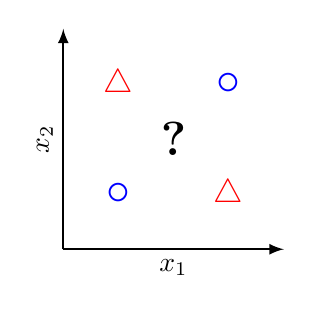
\begin{tikzpicture}[thick, >={latex}, scale=1.4]
		\draw[->] (0, 0) -- node[below] {$x_1$} (2, 0);
		\draw[->] (0, 0) -- node[above, sloped] {$x_2$} (0, 2);
		\node[blue] at (0.5, 0.5) {\LARGE $\bm{\circ}$};
		\node[blue] at (1.5, 1.5) {\LARGE $\bm{\circ}$};
		\node[red] at (0.5, 1.5) {\large $\bm{\bigtriangleup}$};
		\node[red] at (1.5, 0.5) {\large $\bm{\bigtriangleup}$};
		\node[] at (1, 1) {\LARGE \textbf{?}};
	\end{tikzpicture}
\end{center}
Pour palier à ce problème on construit un réseau de neurones en ajoutant une couche cachée.
\begin{center}
	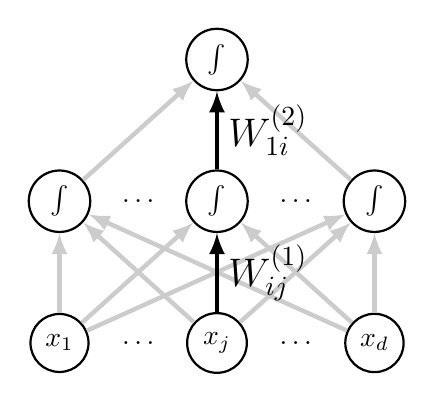
\begin{tikzpicture}[thick, >={latex}]
		\node[draw, circle] (a) at (0, 0) {$x_1$};
		\node at (1, 0) {$\dots$};
		\node[draw, circle] (b) at (2, 0) {$x_j$};
		\node at (3, 0) {$\dots$};
		\node[draw, circle] (c) at (4, 0) {$x_d$};
		
		\node[draw, circle] (x) at (0, 1.8) {$\int$};
		\node at (1, 1.8) {$\dots$};
		\node[draw, circle] (y) at (2, 1.8) {$\int$};
		\node at (3, 1.8) {$\dots$};
		\node[draw, circle] (z) at (4, 1.8) {$\int$};
		
		\node[draw, circle] (o) at (2, 3.6) {$\int$};
		
		\draw[->, ultra thick, black!20] (a) -- (x);
		\draw[->, ultra thick, black!20] (a) -- (y);
		\draw[->, ultra thick, black!20] (a) -- (z);
		\draw[->, ultra thick, black!20] (b) -- (x);
		\draw[->, ultra thick, black!20] (b) -- (z);
		\draw[->, ultra thick, black!20] (c) -- (x);
		\draw[->, ultra thick, black!20] (c) -- (y);
		\draw[->, ultra thick, black!20] (c) -- (z);
		\draw[->, ultra thick] (b) -- node[right] {\Large $\bm{W_{ij}^{(1)}}$} (y);
		
		\draw[->, ultra thick, black!20] (x) -- (o);
		\draw[->, ultra thick, black!20] (z) -- (o);
		\draw[->, ultra thick] (y) -- node[right] {\Large $\bm{W_{1i}^{(2)}}$} (o);
	\end{tikzpicture}
\end{center}

\paragraph{Multi-classe}
Lorsque que l'on a plus de 2 classes il nous faut un neurone par classe en sortie du réseau. On aimerait aussi que la valeur d'un neurone de sortie corresponde à la probabilité conditionnelle $\Pp(y = c~|~x)$. Pour cela la fonction \textbf{softmax} est couramment utilisée :
$$ \text{softmax}(a) = \left[ \dfrac{\exp(a_1)}{\sum_c \exp(a_c)}, ..., \dfrac{\exp(a_C)}{\sum_c \exp(a_c)} \right] $$
On notera $o$ la fonction d'activation de la dernière couche. Si il y a $L$ couches de neurones cachées alors l'indice de la couche de sortie est $L+1$ \\

\PROP[ (Approximation universelle)]{
	Un réseau de neurones avec seule couche cachée peut approcher n'importe quelle fonction continue avec à une distance aussi faible que l'on souhaite	à condition d'avoir assez de neurones dans la couche cachée.
}

\paragraph{Apprentissage}
Le challenge de l'apprentissage est au niveau du calcul du gradient pour les couches cachées. La page Wikipedia  \href{https://fr.wikipedia.org/wiki/R\%C3\%A9tropropagation_du_gradient}{Rétropropagation du gradient} explique comment obtenir ce gradient.

\sect{Apprentissage profond}

Si on se restreint à l'apprentissage de fonction booléenne il peut être montrer qu'il existe des fonctions qui nécessite un nombre exponentielle de neurones si on utilise qu'une seule couche cachée mais seulement un nombre polynomial de neurones si on utilise plusieurs couches. Cela a motivé les chercheurs à concevoir des réseaux plus profond. Cette pratique a eu du succès en :
\begin{itemize}
	\item Vision par ordinateur
	\item Reconnaissance vocale
	\item Traitement du langage naturel
	\item Conduite automatique
	\item Intelligence artificielle pour les jeux
	\item \dots
\end{itemize}

\paragraph{Pré-entraînement non supervisé}
Il est possible de réduire le nombre d'entrées en faisant de l'apprentissage non supervisé. L'idée est d'entraîner une couche à la fois de manière à satisfaire un critère non supervisé puis de fixer les couches entraînées pour en entraîner de nouvelles. On peut par exemple faire en sorte que la couche entraînée soit capable de récréer son entrée d'origine. Cela revient à faire en sorte que l'information perdue d'une couche à une autre ne soit pas déterminante. C'est ce que font les \href{https://fr.wikipedia.org/wiki/Machine_de_Boltzmann_restreinte}{machines de Boltzmann restreintes}, ou \href{https://fr.wikipedia.org/wiki/Auto-encodeur}{auto-encodeurs}.

\paragraph{Abandon (Dropout)}
L'abandon est une technique qui consiste à mettre la valeur de neurones choisis aléatoirement à 0. Cela permet plus de robustesse dans le réseau et permet aussi d'éviter l'overfitting.

\paragraph{Réseaux de neurones convolutifs}
Au lieu d'avoir des poids différents pour toutes les paires de neurones on peut utiliser des filtres de convolution. Pour chaque position possible du filtre sur la couche précédente, on crée un neurone. Et les poids du filtre de convolution sont les même pour tous les neurones crées. Afin de limiter le temps de calculs on rajoute de temps en temps des étapes de sous-échantillonnage (subsampling) qui consistent à moyenner des carrés de neurones afin de réduire leur nombre. Il arrive aussi d'utiliser des étapes de regroupement (pooling) différentes du moyennage. On peut par exemple prendre la valeur maximale ou choisir une valeur aléatoire.
\begin{center}
	\includegraphics[scale=0.4]{conv.png}
\end{center}